\documentclass{article}

\usepackage[fleqn]{amsmath}
\usepackage{amssymb}
\usepackage{graphicx}
\usepackage{tasks} %allows nice lists https://tex.stackexchange.com/a/324740
\usepackage{wrapfig}

\unitlength 1cm
\textheight 22cm
\textwidth 17cm
\oddsidemargin -0.5cm
\evensidemargin -0.5cm
\topmargin -1.5cm
\topskip 0cm
\headheight 0.5cm
\headsep 1cm
\marginparwidth 1.2cm

%%%%%%%%%%%%%%%%%%%%%%%%%%%%% Tasks
\settasks{label-format={\color{green!70!black}\large\bfseries}, label-align=center, label-offset={5mm}, label-width={10mm}, item-indent={2mm}, item-format={\scshape\small}, column-sep={3mm}, after-item-skip=-1mm, after-skip={3mm}
}
%%%%%%%%%%%%%%%%%%%%%%%%%%%%%

\def\R{\mathbb{R}}
\def\Q{\mathbb{Q}}

\begin{document}

\begin{center}
\Large Honors Precalculus Summer Quiz 2
\end{center}

\textbf{Interval, Set Builder, and Roster may be used.  You will be graded on the proper use of each.}

\begin{enumerate}

			\item Evaluate each expression using the functions given.
		
			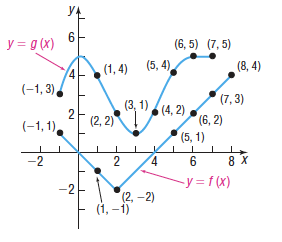
\includegraphics[width=.6\textwidth]{images/hw17}
			
			\begin{enumerate}
				\item $(f \circ g)(1)$
				\item $(f \circ g)(2)$
				\item $(g \circ g)5)$
			\end{enumerate}
								
		\item Suppose that a company has just purchased a new sound system for \$3000. The company chooses to depreciate the sound system using the straight-line method over 3 years.
		
			\begin{enumerate}
				\item Write a linear model that expresses the book value $V$ of
the sound system as a function of its age $x$.
				\item What is the implied domain of the function found in part (a)?
				\item Sketch a graph of the linear function.
				\item What is the book value of the sound system after 2 years?
				\item When will the sound system have a book value of \$2000?
			\end{enumerate}
						
\end{enumerate}

\end{document}